\documentclass[aspectratio=169]{beamer}
\usetheme{Madrid}
\usecolortheme{default}
\usepackage{graphicx}
\usepackage{listings}
\usepackage{tikz}
\usepackage{xcolor}
\usepackage{amsmath}
\usepackage{fontawesome5}
\usetikzlibrary{shapes,arrows,positioning,calc}

% Custom colors
\definecolor{darkblue}{RGB}{0,82,155}
\definecolor{lightblue}{RGB}{80,150,220}
\definecolor{darkgreen}{RGB}{0,128,0}
\definecolor{darkred}{RGB}{180,0,0}

\setbeamercolor{structure}{fg=darkblue}
\setbeamercolor{frametitle}{bg=darkblue,fg=white}

% Code listing style
\lstset{
    basicstyle=\ttfamily\small,
    keywordstyle=\color{darkblue}\bfseries,
    commentstyle=\color{darkgreen},
    stringstyle=\color{darkred},
    showstringspaces=false,
    breaklines=true,
    frame=single,
    numbers=left,
    numberstyle=\tiny\color{gray}
}

\title{Secure File Transfer System}
\subtitle{RSA + AES Hybrid Encryption Protocol}
\author{Systems and Network Security Project}
\institute{University Project}
\date{\today}

\begin{document}

% Title slide
\begin{frame}
\titlepage
\end{frame}

% Table of contents
\begin{frame}{Outline}
\tableofcontents
\end{frame}

% Section 1: Problem Description
\section{Problem Description}

\begin{frame}{The Challenge: Secure File Storage}
\begin{block}{Problem Statement}
\textbf{How do we encrypt files when saving them on a remote server?}
\begin{itemize}
    \item Files need to be stored securely on the server
    \item The encryption key is \textbf{not known in advance}
    \item Each client session should have a unique encryption key
    \item Must prevent unauthorized access to stored files
\end{itemize}
\end{block}

\vspace{0.5cm}

\begin{alertblock}{Security Requirements}
\begin{itemize}
    \item \textbf{Confidentiality}: Only authorized parties can read files
    \item \textbf{Integrity}: Detect any tampering with encrypted data
    \item \textbf{Key Exchange}: Securely share symmetric keys without prior setup
\end{itemize}
\end{alertblock}
\end{frame}

% Section 2: Solution Overview
\section{Encryption Scheme}

\begin{frame}{Solution: Hybrid Encryption (RSA + AES)}
\begin{columns}
\column{0.5\textwidth}
\textbf{Why Hybrid?}
\begin{itemize}
    \item \textcolor{darkblue}{\faKey~RSA (Asymmetric)}
    \begin{itemize}
        \item Secure key exchange
        \item No pre-shared secrets
        \item 2048-bit keys
    \end{itemize}
    \vspace{0.3cm}
    \item \textcolor{darkgreen}{\faLock~AES (Symmetric)}
    \begin{itemize}
        \item Fast data encryption
        \item 256-bit keys
        \item GCM mode (authenticated)
    \end{itemize}
\end{itemize}

\column{0.5\textwidth}
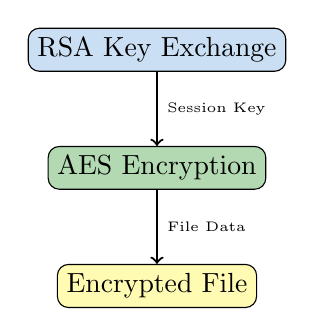
\begin{tikzpicture}[node distance=1.5cm]
    \node[draw, rectangle, rounded corners, fill=lightblue!30] (rsa) {RSA Key Exchange};
    \node[draw, rectangle, rounded corners, fill=darkgreen!30, below of=rsa] (aes) {AES Encryption};
    \node[draw, rectangle, rounded corners, fill=yellow!30, below of=aes] (file) {Encrypted File};
    
    \draw[->, thick] (rsa) -- node[right] {\tiny Session Key} (aes);
    \draw[->, thick] (aes) -- node[right] {\tiny File Data} (file);
\end{tikzpicture}
\end{columns}
\end{frame}

\begin{frame}{Encryption Details}
\begin{block}{RSA-OAEP (Key Exchange Only)}
\begin{itemize}
    \item \textbf{Algorithm}: RSA with OAEP padding
    \item \textbf{Key Size}: 2048 bits
    \item \textbf{Hash Function}: SHA-512
    \item \textbf{Purpose}: Encrypt and transmit AES session key
\end{itemize}
\end{block}

\vspace{0.5cm}

\begin{block}{AES-256-GCM (Data Encryption)}
\begin{itemize}
    \item \textbf{Algorithm}: AES in Galois/Counter Mode
    \item \textbf{Key Size}: 256 bits (32 bytes)
    \item \textbf{Nonce Size}: 12 bytes (unique per encryption)
    \item \textbf{Authentication Tag}: 128 bits (16 bytes)
    \item \textbf{Benefits}: Provides both confidentiality and integrity
\end{itemize}
\end{block}
\end{frame}

\begin{frame}{AES-GCM Message Format}
\begin{center}
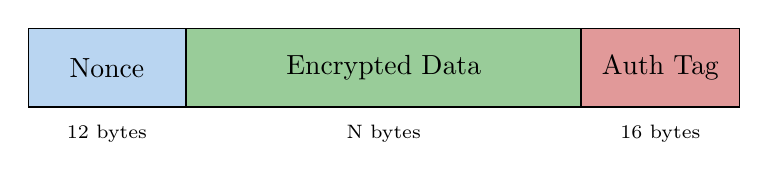
\begin{tikzpicture}
    % Message format boxes
    \node[draw, rectangle, minimum width=2cm, minimum height=1cm, fill=lightblue!40] (nonce) {Nonce};
    \node[draw, rectangle, minimum width=5cm, minimum height=1cm, fill=darkgreen!40, right=0cm of nonce] (cipher) {Encrypted Data};
    \node[draw, rectangle, minimum width=2cm, minimum height=1cm, fill=darkred!40, right=0cm of cipher] (tag) {Auth Tag};
    
    % Labels below
    \node[below=0.1cm of nonce] {\scriptsize 12 bytes};
    \node[below=0.1cm of cipher] {\scriptsize N bytes};
    \node[below=0.1cm of tag] {\scriptsize 16 bytes};
\end{tikzpicture}
\end{center}

\vspace{0.5cm}

\begin{itemize}
    \item \textbf{Nonce}: Random value prepended to ciphertext
    \item \textbf{Encrypted Data}: AES-encrypted file content
    \item \textbf{Authentication Tag}: Verifies data integrity
\end{itemize}
\end{frame}

% Section 3: Protocol Description
\section{Communication Protocol}

\begin{frame}{Protocol Overview}
\begin{block}{Binary Protocol over TCP}
\begin{itemize}
    \item Custom binary format for efficiency
    \item TCP ensures reliable, ordered delivery
    \item Message-based communication
\end{itemize}
\end{block}

\vspace{0.3cm}

\begin{center}
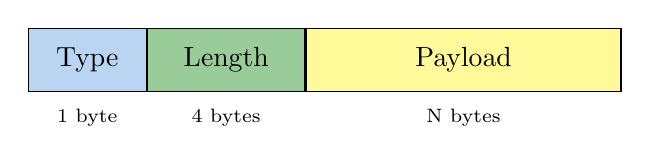
\begin{tikzpicture}
    % Message structure
    \node[draw, rectangle, minimum width=1.5cm, minimum height=0.8cm, fill=lightblue!40] (type) {Type};
    \node[draw, rectangle, minimum width=2cm, minimum height=0.8cm, fill=darkgreen!40, right=0cm of type] (len) {Length};
    \node[draw, rectangle, minimum width=4cm, minimum height=0.8cm, fill=yellow!40, right=0cm of len] (payload) {Payload};
    
    % Labels
    \node[below=0.1cm of type] {\scriptsize 1 byte};
    \node[below=0.1cm of len] {\scriptsize 4 bytes};
    \node[below=0.1cm of payload] {\scriptsize N bytes};
\end{tikzpicture}
\end{center}

\vspace{0.3cm}

\textbf{Message Types:}
\begin{itemize}
    \item \texttt{0x01}: Handshake (RSA key exchange)
    \item \texttt{0x02}: Command (file operations)
    \item \texttt{0x03}: Data (chunked file transfer)
    \item \texttt{0x04}: Response (server replies)
\end{itemize}
\end{frame}

\begin{frame}{Connection Flow}
\begin{center}
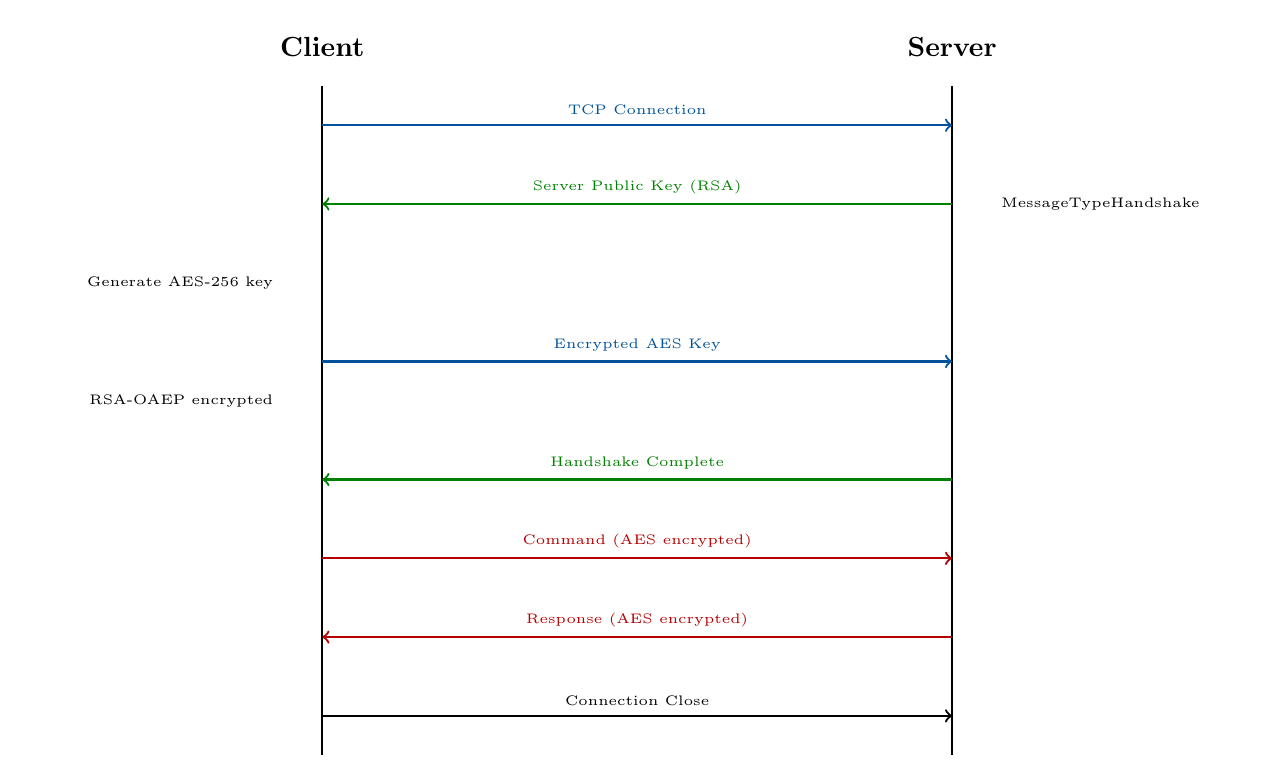
\begin{tikzpicture}[node distance=0.8cm]
    \node (client) at (0,0) {\textbf{Client}};
    \node (server) at (8,0) {\textbf{Server}};
    
    % Connection line
    \draw[thick] (0,-0.5) -- (0,-9);
    \draw[thick] (8,-0.5) -- (8,-9);
    
    % Step 1: TCP Connection
    \draw[->, thick, darkblue] (0,-1) -- node[above] {\tiny TCP Connection} (8,-1);
    
    % Step 2: Server sends public key
    \draw[<-, thick, darkgreen] (0,-2) -- node[above] {\tiny Server Public Key (RSA)} (8,-2);
    \node[right, text width=3cm, font=\tiny] at (8.5,-2) {MessageTypeHandshake};
    
    % Step 3: Client generates AES key
    \node[left, text width=3cm, font=\tiny, align=right] at (-0.5,-3) {Generate AES-256 key};
    
    % Step 4: Client sends encrypted AES key
    \draw[->, thick, darkblue] (0,-4) -- node[above] {\tiny Encrypted AES Key} (8,-4);
    \node[left, text width=3cm, font=\tiny, align=right] at (-0.5,-4.5) {RSA-OAEP encrypted};
    
    % Step 5: Handshake complete
    \draw[<-, thick, darkgreen] (0,-5.5) -- node[above] {\tiny Handshake Complete} (8,-5.5);
    
    % Step 6: Command exchange
    \draw[->, thick, darkred] (0,-6.5) -- node[above] {\tiny Command (AES encrypted)} (8,-6.5);
    \draw[<-, thick, darkred] (0,-7.5) -- node[above] {\tiny Response (AES encrypted)} (8,-7.5);
    
    % Step 7: Close
    \draw[->, thick] (0,-8.5) -- node[above] {\tiny Connection Close} (8,-8.5);
\end{tikzpicture}
\end{center}
\end{frame}

\begin{frame}[fragile]{Handshake Protocol}
\textbf{Step 1: Server $\rightarrow$ Client}
\begin{lstlisting}[language=bash, basicstyle=\ttfamily\footnotesize]
Message Type: 0x01 (Handshake)
Payload: RSA Public Key (PEM format, 2048-bit)
\end{lstlisting}

\vspace{0.3cm}

\textbf{Step 2: Client $\rightarrow$ Server}
\begin{lstlisting}[language=bash, basicstyle=\ttfamily\footnotesize]
Message Type: 0x01 (Handshake)
Payload: AES-256 Key (encrypted with server's public key)
Encryption: RSA-OAEP with SHA-512
\end{lstlisting}

\vspace{0.3cm}

\begin{block}{Result}
Both client and server now share a unique \textbf{AES-256 session key} that will be used to encrypt all subsequent communication.
\end{block}
\end{frame}

% Section 4: Features
\section{Features}

\begin{frame}{Available Commands}
\begin{block}{File Operations}
\begin{description}
    \item[\faUpload~Upload (0x01)] Upload a file to the server (encrypted with AES-256-GCM)
    \item[\faDownload~Download (0x02)] Download a file from the server (chunked transfer)
    \item[\faList~List (0x03)] List all files available in client's directory
    \item[\faTrash~Delete (0x04)] Delete a file from the server
\end{description}
\end{block}

\vspace{0.5cm}

\begin{alertblock}{All Data is Encrypted}
Every file operation encrypts data using the session-specific AES-256-GCM key established during handshake.
\end{alertblock}
\end{frame}

\begin{frame}{Chunked File Transfer}
\textbf{For efficient large file transfers:}

\begin{itemize}
    \item Files are split into chunks (64 KB - 256 KB)
    \item Each chunk includes progress information:
    \begin{itemize}
        \item Chunk index (current chunk number)
        \item Total chunks (how many total)
        \item Chunk size (bytes in this chunk)
        \item Total file size
    \end{itemize}
    \item Adaptive chunk sizing based on file size:
    \begin{itemize}
        \item Small files ($<$ 256 KB): 64 KB chunks
        \item Medium files ($<$ 5 MB): 128 KB chunks
        \item Large files ($\geq$ 5 MB): 256 KB chunks
    \end{itemize}
\end{itemize}

\vspace{0.3cm}

\begin{block}{Benefits}
\faCheck~Memory efficient \quad \faCheck~Progress tracking \quad \faCheck~Network optimization
\end{block}
\end{frame}

\begin{frame}{Command Message Format}
\textbf{Upload Command Example:}

\begin{center}
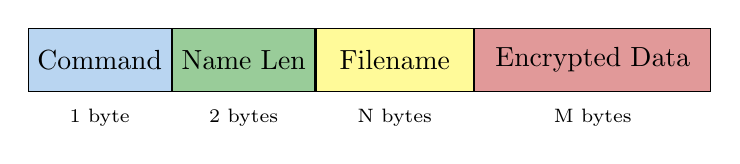
\begin{tikzpicture}
    \node[draw, rectangle, minimum width=1.5cm, minimum height=0.8cm, fill=lightblue!40] (cmd) {Command};
    \node[draw, rectangle, minimum width=1.5cm, minimum height=0.8cm, fill=darkgreen!40, right=0cm of cmd] (flen) {Name Len};
    \node[draw, rectangle, minimum width=2cm, minimum height=0.8cm, fill=yellow!40, right=0cm of flen] (fname) {Filename};
    \node[draw, rectangle, minimum width=3cm, minimum height=0.8cm, fill=darkred!40, right=0cm of fname] (data) {Encrypted Data};
    
    \node[below=0.1cm of cmd] {\scriptsize 1 byte};
    \node[below=0.1cm of flen] {\scriptsize 2 bytes};
    \node[below=0.1cm of fname] {\scriptsize N bytes};
    \node[below=0.1cm of data] {\scriptsize M bytes};
\end{tikzpicture}
\end{center}

\vspace{0.5cm}

\textbf{Response Message Format:}

\begin{center}
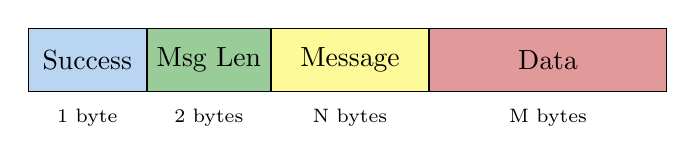
\begin{tikzpicture}
    \node[draw, rectangle, minimum width=1.5cm, minimum height=0.8cm, fill=lightblue!40] (success) {Success};
    \node[draw, rectangle, minimum width=1.5cm, minimum height=0.8cm, fill=darkgreen!40, right=0cm of success] (mlen) {Msg Len};
    \node[draw, rectangle, minimum width=2cm, minimum height=0.8cm, fill=yellow!40, right=0cm of mlen] (msg) {Message};
    \node[draw, rectangle, minimum width=3cm, minimum height=0.8cm, fill=darkred!40, right=0cm of msg] (rdata) {Data};
    
    \node[below=0.1cm of success] {\scriptsize 1 byte};
    \node[below=0.1cm of mlen] {\scriptsize 2 bytes};
    \node[below=0.1cm of msg] {\scriptsize N bytes};
    \node[below=0.1cm of rdata] {\scriptsize M bytes};
\end{tikzpicture}
\end{center}
\end{frame}

% Section 5: Security Aspects
\section{Security Features}

\begin{frame}{Path Traversal Protection}
\begin{block}{Vulnerability: Path Traversal Attack}
Malicious clients might try to access files outside their directory:
\begin{itemize}
    \item \texttt{../../../etc/passwd}
    \item \texttt{/etc/shadow}
    \item \texttt{../../config/private.pem}
\end{itemize}
\end{block}

\vspace{0.3cm}

\begin{exampleblock}{Our Protection Mechanism}
\begin{enumerate}
    \item \textbf{Reject absolute paths}: Only relative paths allowed
    \item \textbf{Clean and resolve paths}: Use \texttt{filepath.Clean()} and \texttt{filepath.Abs()}
    \item \textbf{Verify containment}: Ensure resolved path starts with root directory
    \item \textbf{Reject empty filenames}: Prevent directory access
\end{enumerate}
\end{exampleblock}

\vspace{0.2cm}
\texttt{validatePath()} function ensures all file operations stay within bounds!
\end{frame}

\begin{frame}[fragile]{Path Validation Code}
\begin{lstlisting}[language=Go, basicstyle=\ttfamily\tiny]
func (h *CommandHandler) validatePath(filename string) (string, error) {
    // Reject empty filenames
    if filename == "" {
        return "", fmt.Errorf("filename cannot be empty")
    }
    
    // Reject absolute paths
    if filepath.IsAbs(filename) {
        return "", fmt.Errorf("absolute paths not allowed")
    }
    
    // Get client's root directory
    rootDir, _ := h.getClientDir()
    absRoot, _ := filepath.Abs(rootDir)
    
    // Build and clean full path
    fullPath := filepath.Join(absRoot, filename)
    cleanPath := filepath.Clean(fullPath)
    absPath, _ := filepath.Abs(cleanPath)
    
    // Ensure path is within root directory
    if !strings.HasPrefix(absPath, absRoot+string(filepath.Separator)) {
        return "", fmt.Errorf("path traversal detected")
    }
    
    return absPath, nil
}
\end{lstlisting}
\end{frame}

\begin{frame}{Per-Client Session Storage}
\begin{block}{Isolation Strategy}
Each client gets a unique directory based on their session key:
\begin{enumerate}
    \item Compute SHA-256 hash of the AES session key
    \item Use first 16 hex characters as directory name
    \item Create directory: \texttt{data/<client\_hash>/}
    \item All file operations restricted to this directory
\end{enumerate}
\end{block}

\vspace{0.3cm}

\begin{columns}
\column{0.5\textwidth}
\textbf{Benefits:}
\begin{itemize}
    \item \faCheck~Client isolation
    \item \faCheck~No shared storage
    \item \faCheck~Session-based access
    \item \faCheck~Automatic organization
\end{itemize}

\column{0.5\textwidth}
\begin{exampleblock}{Example}
\texttt{data/}\\
\quad\texttt{1e8130cada7a548b/}\\
\quad\texttt{a30155fdb2c96dab/}\\
\quad\texttt{c45ff82a901b43ef/}
\end{exampleblock}
\end{columns}
\end{frame}

\begin{frame}{Additional Security Features}
\begin{enumerate}
    \item \textbf{Authenticated Encryption}
    \begin{itemize}
        \item AES-GCM provides both encryption and authentication
        \item Any tampering with ciphertext is detected
        \item 128-bit authentication tag prevents forgery
    \end{itemize}
    
    \vspace{0.3cm}
    
    \item \textbf{Unique Nonces}
    \begin{itemize}
        \item Each encryption operation uses a fresh 12-byte nonce
        \item Prevents replay attacks
        \item Cryptographically secure random generation
    \end{itemize}
    
    \vspace{0.3cm}
    
    \item \textbf{Session-Based Keys}
    \begin{itemize}
        \item New AES key for each connection
        \item Keys never stored on disk
        \item Limits impact of key compromise
    \end{itemize}
\end{enumerate}
\end{frame}

\begin{frame}{Security Analysis}
\begin{block}{\textcolor{darkgreen}{Implemented Protections}}
\begin{itemize}
    \item[\faCheck] RSA-2048 for secure key exchange
    \item[\faCheck] AES-256-GCM for authenticated encryption
    \item[\faCheck] Path traversal prevention
    \item[\faCheck] Per-client storage isolation
    \item[\faCheck] Unique nonces for each encryption
    \item[\faCheck] Session-based encryption keys
\end{itemize}
\end{block}

\vspace{0.3cm}

\begin{alertblock}{\textcolor{darkred}{Potential Improvements}}
\begin{itemize}
    \item[\faTimes] No mutual authentication (vulnerable to MITM)
    \item[\faTimes] No perfect forward secrecy (same RSA key reused)
    \item[\faTimes] No replay protection (no sequence numbers)
    \item[\faTimes] No user authentication system
\end{itemize}
\end{alertblock}
\end{frame}

% Section 6: Demo
\section{Demo}

\begin{frame}[fragile]{Demo: Starting the Server}
\textbf{Build and run the server:}
\begin{lstlisting}[language=bash, basicstyle=\ttfamily\footnotesize]
# Build the server
make server
# OR
go build -o bin/server cmd/server/main.go

# Run server with default settings (localhost:8080)
./bin/server

# Run with custom port
./bin/server -port 9000

# Run with custom host and data directory
./bin/server -host 0.0.0.0 -port 8080 -root-dir data
\end{lstlisting}

\vspace{0.3cm}

\textbf{Server automatically:}
\begin{itemize}
    \item Generates RSA keys (if not exist)
    \item Creates data directories
    \item Sets proper permissions
\end{itemize}
\end{frame}

\begin{frame}[fragile]{Demo: Client Usage}
\textbf{Build and connect to server:}
\begin{lstlisting}[language=bash, basicstyle=\ttfamily\footnotesize]
# Build the client
make client
# OR
go build -o bin/client cmd/client/main.go

# Connect to server
./bin/client -host localhost -port 8080
\end{lstlisting}

\vspace{0.3cm}

\textbf{Available commands:}
\begin{lstlisting}[basicstyle=\ttfamily\footnotesize]
> upload myfile.txt        # Upload a file
> download myfile.txt      # Download a file
> list                     # List all files
> delete myfile.txt        # Delete a file
> help                     # Show help
> exit                     # Disconnect
\end{lstlisting}
\end{frame}

\begin{frame}[fragile]{Demo: Interactive Session}
\begin{lstlisting}[basicstyle=\ttfamily\tiny]
$ ./bin/client -host localhost -port 8080

Connected to server successfully!
Handshake completed. Session secured with AES-256-GCM.

Available commands: upload, download, list, delete, help, exit

> upload test.txt
File 'test.txt' uploaded successfully

> list
Files on server:
test.txt

> download test.txt output.txt
Downloading file in chunks...
[====================================] 100%
File downloaded to 'output.txt' (1024 bytes)

> delete test.txt
Are you sure you want to delete 'test.txt'? (y/n): y
File 'test.txt' deleted successfully

> exit
Goodbye!
\end{lstlisting}
\end{frame}

\begin{frame}{System Architecture Diagram}
\begin{center}
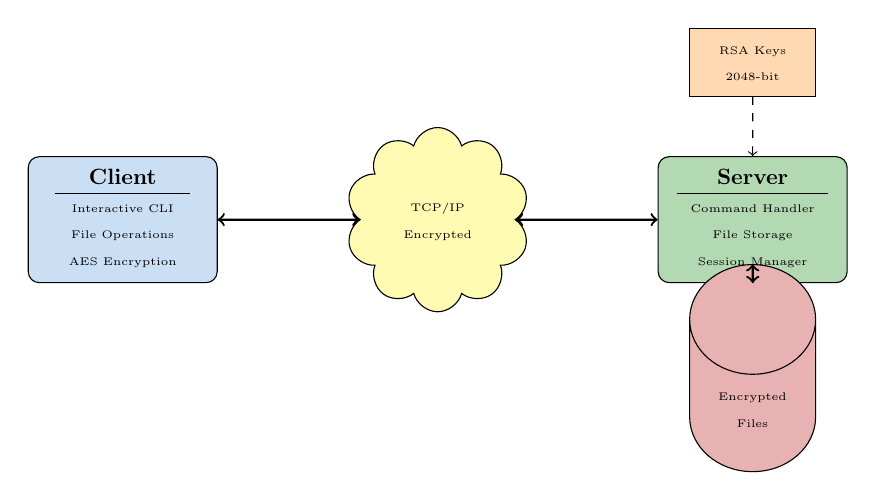
\begin{tikzpicture}[scale=0.8, every node/.style={scale=0.8}]
    % Client box
    \node[draw, rectangle, rounded corners, minimum width=3cm, minimum height=2cm, fill=lightblue!30] (client) at (0,0) {
        \begin{tabular}{c}
        \textbf{Client} \\
        \hline
        \tiny Interactive CLI \\
        \tiny File Operations \\
        \tiny AES Encryption
        \end{tabular}
    };
    
    % Network
    \node[draw, cloud, cloud puffs=10, minimum width=2cm, minimum height=1cm, fill=yellow!30] (network) at (5,0) {
        \begin{tabular}{c}
        \tiny TCP/IP \\
        \tiny Encrypted
        \end{tabular}
    };
    
    % Server box
    \node[draw, rectangle, rounded corners, minimum width=3cm, minimum height=2cm, fill=darkgreen!30] (server) at (10,0) {
        \begin{tabular}{c}
        \textbf{Server} \\
        \hline
        \tiny Command Handler \\
        \tiny File Storage \\
        \tiny Session Manager
        \end{tabular}
    };
    
    % Storage
    \node[draw, cylinder, minimum width=2cm, minimum height=1.5cm, fill=darkred!30, shape border rotate=90] (storage) at (10,-3) {
        \begin{tabular}{c}
        \tiny Encrypted \\
        \tiny Files
        \end{tabular}
    };
    
    % Keys
    \node[draw, rectangle, minimum width=2cm, minimum height=1cm, fill=orange!30] (rsakey) at (10,2.5) {
        \begin{tabular}{c}
        \tiny RSA Keys \\
        \tiny 2048-bit
        \end{tabular}
    };
    
    % Arrows
    \draw[<->, thick] (client) -- (network);
    \draw[<->, thick] (network) -- (server);
    \draw[<->, thick] (server) -- (storage);
    \draw[->, dashed] (rsakey) -- (server);
\end{tikzpicture}
\end{center}
\end{frame}

% Conclusion
\section{Conclusion}

\begin{frame}{Summary}
\begin{block}{Project Achievements}
\begin{itemize}
    \item \textbf{Secure file transfer system} with hybrid encryption
    \item \textbf{RSA-2048 + AES-256-GCM} for key exchange and data encryption
    \item \textbf{Custom binary protocol} over TCP for efficiency
    \item \textbf{Complete command set}: upload, download, list, delete
    \item \textbf{Security features}: path traversal protection, per-client isolation
    \item \textbf{Optimized transfers}: chunked download with progress tracking
\end{itemize}
\end{block}

\vspace{0.5cm}

\begin{alertblock}{Key Takeaways}
\begin{itemize}
    \item Hybrid encryption combines best of symmetric and asymmetric crypto
    \item Proper input validation is critical for server security
    \item Session-based isolation prevents unauthorized access
    \item Authenticated encryption (GCM) provides confidentiality + integrity
\end{itemize}
\end{alertblock}
\end{frame}

\begin{frame}{Future Enhancements}
\begin{enumerate}
    \item \textbf{Mutual Authentication}
    \begin{itemize}
        \item Certificate-based authentication
        \item Prevent man-in-the-middle attacks
    \end{itemize}
    
    \item \textbf{Perfect Forward Secrecy}
    \begin{itemize}
        \item Implement ephemeral Diffie-Hellman key exchange
        \item Protect past sessions if keys compromised
    \end{itemize}
    
    \item \textbf{User Management}
    \begin{itemize}
        \item Multi-user support with authentication
        \item Role-based access control
    \end{itemize}
    
    \item \textbf{Performance Optimizations}
    \begin{itemize}
        \item Parallel chunk transfers
        \item Compression before encryption
        \item Resume interrupted transfers
    \end{itemize}
\end{enumerate}
\end{frame}

\begin{frame}{Technologies Used}
\begin{columns}
\column{0.5\textwidth}
\textbf{Programming Language:}
\begin{itemize}
    \item Go (Golang) 1.21+
\end{itemize}

\vspace{0.3cm}

\textbf{Cryptography:}
\begin{itemize}
    \item \texttt{crypto/rsa}: RSA key generation
    \item \texttt{crypto/aes}: AES encryption
    \item \texttt{crypto/cipher}: GCM mode
    \item \texttt{crypto/sha256}: Hashing
    \item \texttt{crypto/sha512}: RSA-OAEP
\end{itemize}

\column{0.5\textwidth}
\textbf{Networking:}
\begin{itemize}
    \item \texttt{net}: TCP socket programming
    \item \texttt{bufio}: Buffered I/O
\end{itemize}

\vspace{0.3cm}

\textbf{Utilities:}
\begin{itemize}
    \item \texttt{go.uber.org/zap}: Structured logging
    \item \texttt{encoding/binary}: Binary protocol
    \item \texttt{filepath}: Path manipulation
\end{itemize}
\end{columns}

\vspace{0.5cm}

\begin{center}
\textbf{Repository Structure:} Well-organized Go project with \texttt{cmd/}, \texttt{pkg/}, and clear separation of concerns
\end{center}
\end{frame}

\begin{frame}
\centering
\Huge Thank You!

\vspace{1cm}

\Large Questions?

\vspace{1cm}

\normalsize
\textbf{Secure File Transfer System}\\
RSA + AES Hybrid Encryption

\vspace{0.5cm}

\faGithub~github.com/lcensies/ssnproj
\end{frame}

\end{document}
